\documentclass[output=paper,colorlinks,citecolor=brown]{langscibook}
\ChapterDOI{10.5281/zenodo.17158174}

\author{Manfred Krifka\orcid{0000-0002-9610-8352}\affiliation{Leibniz-Zentrum Allgemeine Sprachwissenschaft (ZAS), Humboldt-Universität zu Berlin} and Tue Trinh\orcid{0000-0002-6362-0974}\affiliation{Leibniz-Zentrum Allgemeine Sprachwissenschaft}}
 
\title{Introduction}

\abstract{}

\IfFileExists{../localcommands.tex}{
   \addbibresource{../localbibliography.bib}
   % add all extra packages you need to load to this file

\usepackage{tabularx,multicol}
\usepackage{url}
\urlstyle{same}

\usepackage{listings}
\lstset{basicstyle=\ttfamily,tabsize=2,breaklines=true}

\usepackage{langsci-basic}
\usepackage{langsci-optional}
\usepackage{langsci-lgr}
\usepackage{langsci-osl}
% \usepackage{./langsci/styles/langsci-lgr}
% \usepackage{./langsci/styles/langsci-osl}
% \usepackage{langsci-gb4e}

\usepackage{tikz}
\usetikzlibrary{patterns,calc}
\pgfdeclarepatternformonly{south east lines}{\pgfqpoint{-0pt}{-0pt}}{\pgfqpoint{3pt}{3pt}}{\pgfqpoint{3pt}{3pt}}{
    \pgfsetlinewidth{0.6pt}
    \pgfpathmoveto{\pgfqpoint{0pt}{3pt}}
    \pgfpathlineto{\pgfqpoint{3pt}{0pt}}
    \pgfpathmoveto{\pgfqpoint{.2pt}{-.2pt}}
    \pgfpathlineto{\pgfqpoint{-.2pt}{.2pt}}
    \pgfpathmoveto{\pgfqpoint{3.2pt}{2.8pt}}
    \pgfpathlineto{\pgfqpoint{2.8pt}{3.2pt}}
    \pgfusepath{stroke}}
    
\usepackage{stmaryrd}
\usepackage{wasysym}
\usepackage{multirow}
\usepackage{caption}
\usepackage{subcaption}
\usepackage{mathrsfs}
\usepackage{qtree}

\usepackage{linguex}


   %pminos do not split footnotes
% \interfootnotelinepenalty=10000 %Footnote in Laporte chapters has to be split SN


%\DeclareIndexNameFormat{default}{%
%\nameparts{#1}%
%\usebibmacro{index:name}%
%{\index[names]}%
%{\namepartfamily}%
%{\namepartgiveni}%
% {}% L1
% {}% L2
%{\namepartprefix}% generates spurious space L3
%{\namepartsuffix}% generates spurious space L4
%}

%  {\DeclareIndexNameFormat{default}{%
%     \usebibmacro{index:name}{\index[names]}{#1}{#3}{#5}{#7}}}

%\DeclareIndexNameFormat{default}{%
%  \usebibmacro{index:name}{\sindex[nom]}{#1}{#3}{#5}{#7}}

%\DeclareIndexNameFormat{default}{%
%  \usebibmacro{index:name}{\sindex[person]}{#1}{#3}{#5}{#7}}
%\DeclareIndexNameFormat{default}{%
%\nameparts{#1} \usebibmacro{index:name}{\sindex[person]]}{\namepartfamily}{‌​\namepartgiven}{\nam‌​epartprefix}{\namepa‌​rtsuffix}}

%\newcommand{\smiley}{:)}

%\renewbibmacro*{index:name}[5]{%
%\usebibmacro{index:entry}{#1}%
%{\iffieldundef{usera}{}{\thefield{usera}\actualoperator}\mkbibindexname{#2}{#3}{#4}{#5}}}

% \newcommand{\noop}[1]{}

%remove for final
%\overfullrule=1mm

\newcommand{\tobi}[2]}}
\renewcommand{\S}[1]{\tobi{#1}{\textsc{*}}}

% this volume references
% puts: [this volume]
% already defined: \citetv
%\newcommand{\citepv}[1]{(\citeauthor{#1} \citeyear*{#1} [this volume])}
\newcommand{\citealtv}[1]{\citeauthor{#1} \citeyear*{#1} [this volume]}

%parentheses around example number
\newcommand{\pref}[1]{(\ref{#1})}

% in-text examples

\newcommand{\lnex}[1]{\textit{#1}} %target lang word
\newcommand{\lnlit}[1]{(lit.: `#1')} %literal reading
\newcommand{\lnlat}[1]{(#1)} % latinization
\newcommand{\lntrans}[1]{`#1'} %translation
\newcommand{\lnexl}[2]%
{\lnex{#1}{} \lnlat{#2}} % ex with latinization
\newcommand{\lnexlat}[3]{\lnex{#1}{} \lnlat{#2}{} \lntrans{#3}} % ex with latinization and tranl.

%ch01
\newcommand{\co}[1]{\mbox{\textbf{#1}}}

%ch09

\newcommand{\cyrbulg}[1]{\begin{otherlanguage*}{bulgarian}#1\end{otherlanguage*}}


%ch10
\newcommand{\nlp}{{\small NLP}}
\newcommand{\mwe}{{\small MWE}}
\newcommand{\rae}{{\small RAE}}
\newcommand{\lvc}{{\small LVC}}
\newcommand{\pos}{{\small P}o{\small S}}
%\newcommand{\todo}[1]{ \textcolor{red}{#1} }

%\renewcommand{\labelenumi}{\theenumi}
%\ainamefmt{{vv}{ll}{, ff}{, jj}} % fullname

\newcommand{\biberror}[1]{{\color{red}#1}}

\newcommand{\osenovaitem}{--~}
   %% hyphenation points for line breaks
%% Normally, automatic hyphenation in LaTeX is very good
%% If a word is mis-hyphenated, add it to this file
%%
%% add information to TeX file before \begin{document} with:
%% %% hyphenation points for line breaks
%% Normally, automatic hyphenation in LaTeX is very good
%% If a word is mis-hyphenated, add it to this file
%%
%% add information to TeX file before \begin{document} with:
%% %% hyphenation points for line breaks
%% Normally, automatic hyphenation in LaTeX is very good
%% If a word is mis-hyphenated, add it to this file
%%
%% add information to TeX file before \begin{document} with:
%% \include{localhyphenation}
\hyphenation{
    Beck-man
    Ngu-yen
    back-chan-nel
    back-chan-nels
    mo-not-o-nous
    ste-reo-typ-i-cal
}

\hyphenation{
    Beck-man
    Ngu-yen
    back-chan-nel
    back-chan-nels
    mo-not-o-nous
    ste-reo-typ-i-cal
}

\hyphenation{
    Beck-man
    Ngu-yen
    back-chan-nel
    back-chan-nels
    mo-not-o-nous
    ste-reo-typ-i-cal
}

   \boolfalse{bookcompile}
   \togglepaper[23]%%chapternumber
}{}

\begin{document}
\maketitle

\section{Biased questions: An overview}

According to the standard analysis of question meaning, a question denotes a set of propositions, i.e. those that answer the question. Polar questions, the subject matter of this volume, are taken by many theorists to denote a set of their positive and negative answers \citep{hamblin1973questions, groenendijk1984semantics, ciardelli2019inquisitive}.\footnote{There are non-trivial differences in how these theories of question semantics arrive at the set of propositions in \xref{whetherrainmeaning}, but for now we abstract away from these differences.} For example, \xref{whetherrain} denotes the set of propositions in \xref{whetherrainmeaning}.  

\ea \label{whetherrain}
Is it raining?
\ex \label{whetherrainmeaning}
$\{$it is raining, $\neg$it is raining$\}$
\z

%A wh-question such as \xref{whowon} also denotes a set of propositions. Some take this set to be the set of congruent answers \citep{hamblin1973questions, Rooth:1992}. Assuming, for simplicity, that John and Mary are the only two relevant individuals, this would be as in \xref{congruent}. Others take it to be the set of complete answers, as in \xref{complete} \citep{groenendijk1984semantics}.\footnote{See also \citealt{ciardelli2019inquisitive} for the newer approach, inquisitive semantics.} %A newer approach, ``inquisitive semantics'' \citep{ciardelli2019inquisitive}, also adopts the semantics in \xref{whetherrainmeaning}, and in \xref{congruent}.

%\ex.
%\a.\label{whowon}
%Who won?
%\b.\label{congruent}
%$\{$John won, Mary won$\}$
%\b.\label{complete}
%$\{$only John won, only Mary won, both won, neither won$\}$

%There is an exciting 
%A new approach, ``inquisitive semantics'' \citep{ciardelli2019inquisitive}[DG: reminder to fix reference], differs from the standard view in a number of respects, but significantly, agrees with the latter in what questions mean. Specifically, it also assigns to \xref{whetherrain} the set in \xref{whetherrainmeaning}, and to \xref{whowon} the set in \xref{congruent}.

%From now on we will not be concerned with wh-questions, but instead will focus exclusively on polar questions. 

%What all the theories we just discussed have in 
A common assumption among such theories of polar questions is that the alternatives proposed by the question are balanced, that is, the propositions in the set are equally ranked. This is represented visually in \figref{balanced}.

\begin{figure}
\hspace{0.3cm}$\phi$\hspace{2.9cm}$\neg\phi$\\
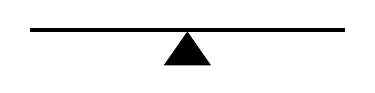
\begin{tikzpicture}
\draw[ultra thick](-2,1) -- (2,1);
\fill[black] (0,0.98) -- (-0.3,0.55) -- (0.3,0.55);
\end{tikzpicture}
\caption{Balanced question}
\label{balanced}
\end{figure}

But as we all know, sometimes questions are biased. For example, the speaker might take one answer to be more likely than another. This leads to an imbalance among the propositions, as in \figref{unbalanced}.

\begin{figure}
%\hspace{0.3cm}\phantom{$\phi$}\\
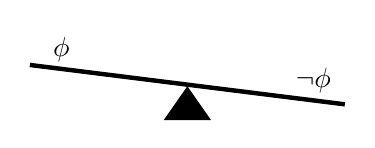
\begin{tikzpicture}[baseline={([yshift={-1ex}]current bounding box.north)}]
\draw[ultra thick](-2,1) -- (2,0.5);
\fill[black] (0,0.73) -- (-0.3,0.3) -- (0.3,0.3);
\node at (-1.6,1.2) {$\phi$};
\node at (1.6,0.8) {$\neg\phi$};
\end{tikzpicture}
\caption{Biased question}
\label{unbalanced}
\end{figure}

There are several interesting questions about this kind of imbalance, including what constitutes the evidence for such an imbalance, whether there are different kinds or different dimensions of tilts, and how can we represent these aspects of meaning.

%\section{Problems for the standard view}

%\subsection{Polar vs. alternative questions}

The existence of biased questions was famously pointed out  by \citet{Bolinger:1978}, who drew attention to the differences between simple polar questions and alternative questions. A polar question like \xref{whetherhelp} is totally normal but an alternative question like \xref{whetherhelpornot} is quite strange, perhaps because the questioner is more interested in the positive answer being true rather than the negative, and this is better expressed by \xref{whetherhelp} than \xref{whetherhelpornot}.

\ea
\ea\label{whetherhelp}
Will you help me?
\ex\label{whetherhelpornot}
Will you help me or not?
\z
\z

Another difference is that polar questions can be conversation starters whereas alternative questions cannot. The sequence in \xref{starter} sounds normal, while that in \xref{nonstarter} sounds odd.

\ea
\ea[]{
Nice to meet you! Do you like to play golf?}\label{starter}
\ex[\#]{
Nice to meet you! Do you like to play golf or not?}\label{nonstarter}
\z
\z

There is also a difference with respect to question complementizers. It seems that embedded polar questions introduced by \textit{if} correlate with simple polar questions, while those introduced by \textit{whether} correlate with alternative questions. Thus, the scenario in \xref{willyoumarryme} is more naturally reported as \xref{ifmarry} than \xref{whethermarry}. 

\ea[]{
John asked Mary: ``Will you marry me?''
}\label{willyoumarryme}
\ex[]{
John asked Mary if she would marry him
}\label{ifmarry}
\ex[?]{
John asked Mary whether she would marry him
}\label{whethermarry}
\z

%John asked Sue if she would marry him is fine, but John asked Sue whether she would marry him seems to indicate that John is neutral about both possibilities, which in this case would make the question sound odd.
Bolinger suggests that the complementizer \textit{whether} is used when the speaker, having already considered the alternative possibilities, is trying to dispassionately gain information about them. We add that this corresponds to our intuition that the use of \emph{whether} in \xref{whethermarry} indicates that John thinks a negative answer is a serious possibility, at least as likely as the positive answer.
%seems to suggest that the subject has no preference with respect to the positive and the negative answer. The complementizer \textit{if}, on the other hand, does not seem to have this inference. %\textcolor{blue}{[DG: My intuition is that the asymmetry here isn't nearly as sharp as for the matrix polar question vs. alternative question. In fact, I think \xref{whethermarry} is basically fine. There is perhaps an intuitive difference, but I wouldn't say that ``whether" conveys that John has ``no preference". It might be that ``whether" conveys that John thinks a negative answer is a serious possibility, though not more likely than the positive answer. Perhaps it conveys that the two answers are equally possible, while ``if" perhaps only draws attention to the positive answer (but doesn't necessarily mean that John is ``biased" for the positive answer).]}

So we see that simple polar questions can highlight one option, while alternative questions highlight both options. We can then ask whether alternative questions are neutral. But as \citet{biezma2019alternative} shows, alternative questions are not neutral. They come with what Biezma calls a `cornering effect': The hearer is forced to give an answer. The question in \xref{marryornot} sounds like it is the last of a series of questions to which the speaker has not gotten a proper answer.

%****DG: I removed the following footnote. This distinction is addressed to a certain extent by Biezma & Rawlins 2017, and Beltrama et al. 2020, who refer to exs like these as "Complement Alternative Questions". Perhaps we'll want to include some discussion of this too, and if so, I can come back and add it. 
%\footnote{This cornering effect seems not to be always present. Consider the following exchange.

%\ex.\label{evenoddexhange}
%\a.[A:] I'm thinking of a number between 1 and 10. Guess which!
%\b.[B:] Is it even or odd?

%Given that a number is either even or odd, B's question is equivalent to an alternative question. However, the question does not have to be read as ``cornering'' A in anyway. \textcolor{blue}{[DG: I thought the cornering effect was only for ``negative alternative questions", which is when the second disjunct is always the negation of the first, e.g. ``or not" or ``or isn't it", etc.]}}

\ea \label{marryornot}
Will you marry me or not?
\z


Let us look at negated questions and the uses of antonyms. Assuming that a bridge is either closed or open, the standard view on questions would assign all of the following sentences the same meaning, namely $\{o, \neg o\}$, where $o$ stands for the bridge is open and $\neg o$ for the bridge is not open, i.e. closed.

\ea\label{bridgequestions}
\ea
Is the bridge open?\label{whetheropen}
\ex \label{openornot}
Is the bridge open or not?
\ex
Is the bridge open or closed?
\ex \label{closed}
Is the bridge closed?
\ex \label{closedornot}
Is the bridge closed or not?
\z
\z

However, the choice of the expression clearly matters \citep{vanrooysafarova2003polar, bustamente2012real, roelofsengool2010disjunctive, trinh2014how}.
In a context where the speaker needs to get to the other side of the river and wants the bridge to be open, and there is no contextual indication as to whether or not it is open, the questions in \xref{bridgequestions} are ranked in the order of most to least appropriate. %, with \xref{whetheropen} being the most appropriate and \xref{closedornot} being the least appropriate. %\textcolor{blue}{[DG: This depends on what else has been said in the context, right? If an interlocutor claims the bridge is closed, and then does or says something to imply it is not closed, the speaker who needs to get to the other side and wants the bridge to be open would then nevertheless find \xref{closedornot} to be most natural, or at least as natural as \xref{whetheropen}.]}

Similarly, in a context where the speaker needs to throw an even number, the utterance in \xref{dice} would be most appropriate with the leftmost choice (\textit{even}) and least appropriate with the rightmost choice (\textit{odd or not}). %\textcolor{blue}{[DG: Suppose the speaker needs an even, but steadfastly believes that their luck is cursed, and therefore an odd number is almost certain. Then ``odd'' is most natural. This comment and my previous comment both are just highlighting the fact that bias has multiple possible sources, as is already mentioned in the chapter above.]}

\ea\label{dice}
I don't dare to look! Is the number even  / $^{?}$even or not / $^{??}$even or odd / \#odd / \#\#odd or not?
\z

However, in both preceding examples, further additions to context can change these intuitions. For example, suppose that in \xref{bridgequestions}, the speaker wants the bridge to be open, but their interlocutor has just indirectly implied that the bridge is closed. In that case, \xref{closed} is most natural. Or suppose the interlocutor ambiguoulsy implies first that it is closed, and then that it is not closed. In that case, \xref{closedornot} would be most natural, despite that the speaker wants the bridge to be open. As for \xref{dice}, suppose the speaker needs an even, but steadfastly believes that their luck is cursed, and therefore an odd number is almost certain. Then asking the question with \textit{odd} is most natural. What this shows is that the contextual factors affecting which question form is most natural are  influenced by multiple competing factors. %All of this shows how sensitive to context the naturalness of the varying forms are. 

How can we differentiate between question meanings so that we can describe their different uses?  Obviously the truth conditional content offered by the theories discussed above does not suffice. We have to look at how these truth conditions are expressed formally. One idea that has been proposed is that different kinds of questions introduce different kinds of discourse referents (DR) (see \citealt{krifka2013} for the role of propositional discourse referents in responses). 

\ea\label{DRs}
\ea \label{rain} 
``Is it raining?'' \hfill $\leadsto$ DR: `it is raining'
\ex\label{notrain}
``Is it not raining?'' \hfill $\leadsto$ DR: `it is not raining'
\ex\label{rainornot}
``Is it raining or not?'' \hfill $\leadsto$ DR: `it is raining', `it is not raining'
\z
\z

As a consequence, these questions would have different discourse potentials. There are other proposals, such as  \citet{roelofsengool2010disjunctive}, which makes it possible to ``highlight'' one of the propositions, leading to a more complex semantic representation. Theories also exist which say the meaning of questions does not have to be balanced. These allow for a monopolar interpretation of questions. Hamblin's semantics, for example, allows for \xref{rain} to denote the set contain only one proposition, namely the proposition that it is raining. The question in  \xref{notrain} would denote the set containing only the proposition that it is not raining. The set denoted by the alternative question in \xref{rainornot} would contain both of these propositions. This is different from the assertion, which is just the proposition, not a set containing the proposition \citep{vanrooysafarova2003polar}.

In commitment space semantics \citep{krifka2015bias}, there is also a way to differentiate between the cases in \xref{DRs}. We assume the common ground, or ``commitment space'', represented by $C$, to be a set of information states, or ``commitment states'', represented by $c$. Each commitment state is a set of possible worlds. The root of C, represented as $\sqrt{C}$, is the set of ``largest'' commitment states, so to speak. %\textcolor{blue}{[DG: In the last draft this said ``smallest'', but I think it should be ``largest'', please double check.]}

\ea\label{rootC}
$\sqrt{C} = \{c \in C \mid \neg\exists c' \in C [c \subset c']\}$
\z

In case of an assertion, say of the proposition that it is raining, represented as $r$, the commitment space C is updated so that it contains only commitment states which entail $r$. 

\ea\label{assertioncommitment}
$C +$ `it is raining' $= \{c \in C \mid c \subseteq r\}$
\z

Questions differ from assertions in that they do not change $\sqrt{C}$, the root of the commitment space. 

\ea\label{questioncommitment}
\ea\label{positivequestioncommitment}
$C +$ `is it raining?' $= \sqrt{C} \cup \{c \in C \mid c \subseteq r\}$
\ex\label{negativequestioncommitment}
$C +$ `is it not raining?' $= \sqrt{C} \cup \{c \in C \mid c \subseteq \neg r\}$
\ex\label{alternativequestioncommitment}
$C +$ `is it raining or not?' $= \sqrt{C} \cup \{c \in C \mid c \subseteq r \vee c \subseteq \neg r\}$
\z
\z

In other words, questions do not add information. Instead, they restrict the continuation of the discourse. As shown in \xref{positivequestioncommitment} and \xref{negativequestioncommitment}, the ``positive'' and the ``negative'' simple polar question restricts $C$ to those $c$ which entail $r$ and $\neg r$, respectively. This is intended to represent the fact that the speaker wants to see if the discourse can continue with the information that it is raining, in the first case, or with the information that it is not raining, in the second case. The alternative question, as shown in \xref{alternativequestioncommitment}, has a yet different meaning from the two simple polar questions.  

Note, however, that this approach would still not capture the distinction between \xref{openornot} and \xref{closedornot}, reproduced below in \xref{openornot2} and \xref{closedornot2}.

\ea\label{openornot2}
Is the bridge open or not?
\ex\label{closedornot2}
Is the bridge closed or not?
\z

The general question, then, is how to represent polar questions properly to capture their different uses.

We now turn to the topic of negation in polar questions \citep{bolinger1957interrogative, Ladusaw:1979, Ladd:1981}. \citet{Ladd:1981} discusses polar questions such as those in \xref{negationquestions}. 

\begin{exe}\label{negationquestions}
\ex\label{lownegation} 
Is it not raining?
\ex\label{highnegation}
Isn't it raining?
\end{exe}

These questions differ with respect to where syntactic negation is. In \xref{lownegation}, it is low, below the subject, while in \xref{highnegation} it is high, above the subject. The low negation question seems to implicate that the speaker wants to be informed as to whether the proposition that it is not raining is true. The high negation question, on the other hand, seems to indicate that the speaker is already inclined to assume that it is raining and wants to confirm this belief.

\citet{Ladd:1981} assumes that high negation questions are actually ambiguous, with both ``outer" and ``inner" interpretations. %Specifically, they allow for a ``low'' interpretation. 
He claims the ambiguity can be resolved by the presence of polarity items like \textit{too} and \textit{either}, which disambiguate the question toward the outer and inner readings respectively. %, or a negative polarity item such as \textit{neither}, which disambiguates the question towards the low reading. %Examples are given in \xref{tooeither}

\begin{exe}\label{tooeither}
\ex\label{too}
Isn't Jane coming too? \hfill $\rightarrow$ outer interpretation
\ex\label{either}
Isn't Jane coming either? \hfill $\rightarrow$ inner interpretation
\end{exe}

A prominent analysis of these facts is proposed by \citet{romerohan2004negative}. %Han:2002a
This analysis assumes a \textsc{verum} operator, whose meaning is a conversational version of the adverbial \textit{for sure}, and whose occurrence is associated with a syntactically preposed high negation. We have the following form-meaning pairs, where $p$ stands for the proposition that Jane is coming. Notice that negation can scope either below or above the \textsc{verum} operator.

\begin{exe}\label{hanromero}
\ex\label{hanromerolowneg}
Is Jane not coming? \\= \textsc{whether}($\neg p$) = $\{\neg p, \neg\neg p\}$ = $\{p, \neg p\}$
\ex\label{hanromerohighnegeither}
Isn't Jane coming (either)? \\ = \textsc{whether}(\textbf{verum}($\neg p$)) = $\{$\textit{for-sure}($\neg p$),  $\neg$\textit{for-sure}($\neg p$)$\}$
\ex\label{hanromerohighnegtoo}
Isn't Jane coming (too)? \\ = \textsc{whether}($\neg$\textbf{verum}($p$)) = $\{$$\neg$\textit{for-sure}($p$), \textit{for-sure}($p$)$\}$
\end{exe}

Romero and Han propose that \textsc{verum} is also present when the question contains the adverb \textit{really}. Thus, \xref{hanromeroreally} ends up having the same meaning as \xref{hanromerohighnegtoo}.

\ea\label{hanromeroreally}
Is Jane really coming?\\
= \textsc{whether}(\textbf{verum}($p$)) = $\{$\textit{for-sure}($p$), $\neg$\textit{for-sure}($p$)$\}$
\z

A similar approach is adopted by \citet{krifka2015bias}, which assumes a commitment operator $\vdash$ that is present in both assertions and questions, and negation can scope either below or above that operator.

\begin{exe}\label{krifkacommitmentoperator}
\ex
$C +$ `is Jane not coming?' = $\sqrt{C} \cup C +$ [Addressee $\vdash$ $\neg p$]\\
$\leadsto$ the speaker is checking whether the addressee is committed to $\neg p$
\ex
$C +$ `isn't Jane coming?' = $\sqrt{C} \cup C +$ $\neg$[Addressee $\vdash$ $p$]\\
$\leadsto$ the speaker is checking whether the addressee is not committed to $p$
\end{exe}

So, there is a wide array of syntactic profiles available for polar question formation: high and low negation, the presence or absence of adverbials like \textit{really}, and also, the presence or absence of bias inducing expressions such as negative polarity items (NPIs). \tabref{tab:1} presents a fine-grained list (probably non-exhaustive) of relevant phenomena (see also the bias profiles discussed in \citealt{gartnergyuris2017delimiting}).

\begin{table}[t]
\fittable{
\begin{tabular}{lll}
\lsptoprule
Example & Abbreviation & Label\\
\midrule
Is it raining? & PQ & positive question\\
Is it not raining? & NQ & negative question\\
Isn't it raining? & HPQ & high negated positive question\\
Isn't it not raining? & HNQ & high negated negated question\\
Is it really raining? & RPQ & \textit{really} positive question\\
It is really not raining? & RNQ & \textit{really} negated question\\
IS it raining? & FPQ & focused positive question\\
IS it not raining? & FNQ & focused negated question\\
Is it REALLY raining? & FRPQ & focused \textit{really} positive question\\
Is it REALLY not raining? & FRNQ & focused \textit{really} negated question\\
It is raining? & DPQ & declarative positive question\\
Is it raining?? & IPQ & incredulity positive question\\
Is it raining or not? & APNQ & alternative question with negation\\
Is the bridge open or closed? & AAntQ & alternative question with antonyms\\
Do you have any potatoes? & npiPQ & positive question with polarity item\\
\lspbottomrule
\end{tabular}
}
\caption{Polar question varieties} \label{tab:1}
\end{table}

Coming back to the topic of negation in questions, one promising approach is to look at contextual features. This goes back to \citet{buringgunlogson2000positive}, which assumes three levels of contextual evidence with respect to the prejacent of a polar question: positive, neutral, and negative. The generalization in \tabref{buringgunlogsongeneralization} is established. 
%\textcolor{blue}{[DG: I'm doubtful that we can get people to adopt the terminology and abbreviations in Table 1.Given that, I think the only reason to  introduce systematic abbreviations here is if we ourselves can consistently use them in the rest of the chapter. But in the following, we display and discuss plots from a few different experiments by other researchers who each have their own different abbreviations, including already ``PPQ" in the next table. So, I suggest that we remove Table 1.]} %Lots of people have worked on this topic now and there is no agreed upon terminology, let alone abbreviations. 

\begin{table}
\begin{tabularx}{\textwidth}{lCCc}
  \lsptoprule
\multirow{2}{*}{contextual evidence} & \multirow{2}{*}{PPQ} & \multicolumn{2}{c}{HPQ} \\
\cmidrule{3-4}
 & {} & high reading & low reading \\
   \midrule
positive & \ding{51} & \ding{55} & \ding{55}\\
neutral & \ding{51} & \ding{51} & \ding{55}\\
negative & \ding{55} & \ding{51} & \ding{51}\\
  \lspbottomrule
\end{tabularx}
\caption{\quotecite{buringgunlogson2000positive} generalization} \label{buringgunlogsongeneralization}
\end{table}

\largerpage[2]
The contextual evidence is ``positive'' if it supports the prejacent, ``neutral'' if it neither supports nor speaks against the prejacent, and ``negative'' when it speaks against the prejacent. Thus, even PPQs are not neutral, in the sense that there are contexts where they cannot be used, namely those with negative evidence. Note that \citet{buringgunlogson2000positive} take HPQ with a low negation to mean the same as NQ. Thus, \xref{hpqlow} and \xref{nq} would be equivalent in this approach.

\ea
\ea\label{hpqlow}
Isn't Jane coming either?
\ex\label{nq}
Is Jane not coming either?
\z
\z

The first experimental work on this topic is done by \citet{roelofsen2013}. This is a rating experiment, which contrasts prior speaker's belief (SB) with positive, neutral, and negative contextual evidence (CE). The experiment yields interesting results about the different uses of positive, high negation, and low negation questions as presented in \figref{pic:123}.
%\textcolor{blue}{[DG: I haven't read this paper, and I guess I need to. The results in (24) and (25) make no sense to me. Either I've misunderstood or there was a problem with the stimuli. Note also that we don't actually discuss this data below, which makes me wonder if we should include these plots. It seems the main reason for mentioning this paper is to discuss the preference rules and OT below, maybe we could just do that directly.]}

\begin{figure}
\subfigure[PPQs]{
\includegraphics[width=.45\textwidth]{figures/Roelofsen-PPQ.pdf}
}
\subfigure[HNPQ]{
\includegraphics[width=.45\textwidth]{figures/Roelofsen-HNPQ.pdf}
}
\subfigure[LNPQ]{
\includegraphics[width=.45\textwidth]{figures/Roelofsen-LNPQ.pdf}
}
\caption{\quotecite{roelofsen2013} experimental results}
\label{pic:123}
\end{figure}


These uses were described in terms of various preference rules. An example of such a rule is ``ask only if needed''. According to this rule, there is no need to ask any question if speaker's belief and contextual evidence coincide. Another rule is ``avoid reversing processes'', which says that it would be strange to ask whether $\neg p$ is true when the speaker's belief or the contextual evidence supports $p$. Yet another rule is ``use the least marked form'', which would prefer a positive question to a negative or an alternative question, for example. We note that these rules resemble constraints in bidirectional optimality theory (OT) in pragmatics, hence raise the question whether bidirectional OT should be employed in analyzing biased questions. We believe this perspective is promising.

It has become consensus to assume three levels -- positive, neutral, negative -- for both contextual evidence and prior speaker's belief, or ``evidential bias'' and ``epistemic bias'', which are terms proposed by \citet{sudo2013biased} which have gained some currency. We could let SB stand for prior speaker's belief and CE for contextual evidence, and use $+$, $0$ and $-$ to represent the three levels positive, neutral, and negative. %Furthermore, we could adopt the convention of placing. 
Bias profiles of questions could then be represented more succinctly. For example, [SB$-$, CE$+$] is a question with negative prior speaker's belief and positive contextual evidence, and [SB$0+$, CE$-$] would be a question with neutral or positive prior speaker's belief and negative contextual evidence. If we adopt the convention of placing the value for SB to the left of that for CE, the profiles can be represented even more economically. Thus, [SB$-$, CE$+$] can be shortened to [$-$/$+$] and [SB$0+$, CE$-$] to [$0+$/$-$]. %\textcolor{blue}{[DG: It looks like maybe we get some use of these abbreviations some of the tables below; maybe we should introduce those abbreviations there.]} 

\citet{domaneschi2017bias} present further experimental results. Tests were conducted on high negation questions (HiNQ), low negation questions (LowNQ), positive question (PosQ), and positive question with \textit{really} (ReallyPosQ). The object languages were English and German. Participants were given a selecting task, where they had to pronounce their option. The main results are presented in \figref{fig:chart23}. %\textcolor{blue}{[DG: With this data as well, we're not really discussing it. Perhaps that is fine, and the idea here is just to provide the reader with the results themselves. But then we need to explain the condition labels on the X axis. If we decide to keep these plots in here, I am happy to add explanations for the condition labels.]}

\begin{figure}
% \begin{subfigure}{0.43\textwidth}\centering
\includegraphics[height=.45\textheight]{figures/Domaneschi-1.pdf}
%\caption{\color{red}{Please provide a caption}}
%\label{fig:chart2}
% \end{subfigure}
% \begin{subfigure}{0.41\textwidth}\centering
\includegraphics[height=.45\textheight]{figures/Domaneschi-2.pdf}
%\caption{\color{red}{Please provide a caption}}
%\label{fig:chart3}
% \end{subfigure}
\caption{\quotecite{domaneschi2017bias} experimental results}
\label{fig:chart23}
\end{figure}

A recurring question is whether syntactically high negation questions (HPQs) are semantically ambiguous. \citet{Ladd:1981} claims that they are; \citet{sailor2012remarks, anderbois2019, goodhue2022} all argue that they are not. It should be pointed out, however, that Sailor's data can be accounted for by assuming that for English, HPQs are ambiguous while NQs are not, and for German, the opposite is the case. %\textcolor{blue}{[DG: I'm not sure what is meant by this claim. In my paper, I make a concerted effort to show that the data speaks against the existence of an ambiguity in American English HPQs.]}

\ea English
\ea Isn't there a train in the early morning? \hfill $\neg Qp$ / $Q\neg p$
\ex Is there no train in the early morning? \hfill $Q \neg p$
\z

\ex German
\ea Gibt es hier nicht einen Zug am Morgen? \hfill $\neg Qp$
\ex Gibt es hier keinen Zug am Morgen? \hfill $Q\neg p$ / $\neg Qp$
\z
\z

How can we explain this difference between English and German? Suppose we say that in the [SB$+$, CE$-$] scenario, the wide-scope negation reading is the best. If we then assume that in German this wide-scope interpretation can also be expressed by a syntactically low negation, we can explain why there is more uses of this option in German.

The interesting issue here, therefore, is whether there are different readings of high negation questions and low negation questions. 

\citet{sudo2013biased} looks at the Japanese counterparts of positive questions (PQs), high negation questions (HQs), and low negation questions (NQs). 

\ea
\gll Mary-ga kita $\{\emptyset$ / no / desho$\}$\\
Mary-NOM came\\ 
\glt `Did Mary come' \hfill PQ 
\ex
\gll doko-ka nihon-shoku nai?\\
where-\textsc{ka} Japanese-food not.exist\\
\glt `Isn't there some Japanese restaurant?' \hfill HQ
\ex
\gll doko-mo nihon-shoku nai?\\
where-\textsc{mo} Japanese-food not.exist\\
\glt `Isn't there any Japanese restaurant?' \hfill NQ
\z

Sudo treats epistemic and evidential bias, at different levels, as features which can be combined in different ways as presented in \tabref{figtab:chart45}. \citet{gyuris2017new} looks at three different types of polar questions in Hungarian as presented in \tabref{figtab:chart6}.

\begin{table}
% \includegraphics[width=.5\textwidth]{figures/Sudo-1.pdf}
\caption{\quotecite{sudo2013biased} taxonomy}
\label{figtab:chart45}
\begin{tabularx}{\textwidth}{XXXc}
\lsptoprule
 Question type & Epistemic &  Evidential & Short\\
 \midrule
 PQ            & none      &  not negative &  --0+/0+\\
 HQ            & positive  &  not positive & +/--0\\
NQ             &  positive & neutral        & +/0\\
\lspbottomrule
\end{tabularx}
\end{table}

\begin{table}
% \includegraphics[height=.5\textheight]{figures/Gyuris-1.pdf}
\caption{\quotecite{gyuris2017new} taxonomy}
\label{figtab:chart6}
\fittable{
\begin{tabular}{lccc}
\lsptoprule
                                  & -e-interrogative &  $\wedge$-interrogative  & $\wedge$-declarative\\
                                  \midrule
Neutral information question, (11)& {\langscicheckmark} & {\langscicheckmark} & {\langscicross}\\
Grounding question, (12)          & {\langscicross}     &\%                   & {\langscicheckmark}\\
Indirect Request                  & {\langscicross}     &  {\langscicheckmark}& {\langscicross}\\
Indirect offer, (14)              & {\langscicheckmark} &  {\langscicheckmark}& {\langscicross} \\
 Conversation  starter, (15)      & {\langscicross}     &  {\langscicheckmark}& {\langscicross}\\
Pedagogical question              & {\langscicheckmark} & {\langscicheckmark} & {\langscicross}\\
Monological question              & {\langscicheckmark} & {\langscicheckmark} & {\langscicross}\\
Exam question, (18)               & {\langscicheckmark} & {\langscicheckmark} & {\langscicross}\\
Rhetorical question, (19)         & {\langscicheckmark} & {\langscicheckmark} & {\langscicross}\\
\lspbottomrule
\end{tabular}
}
\end{table}

\begin{table}
% \includegraphics[height=.17\textheight]{figures/Gyuris-2.pdf}
\caption{\quotecite{gartnergyuris2017delimiting} bias profiles}
\label{figtab:chart7}
 \begin{tabularx}{.8\textwidth}{Xcc}
 \lsptoprule
 Question type & Speaker belief & Current evidence\\
 \midrule
  ePQ          &                 &0                        \\
 $\wedge$PQ          &                 &0, for some speakers --  \\
 $\wedge$DPQ         &                 &+                        \\
 eHQ           &   +             &0                        \\
 $\wedge$HQ          &   +             &--0                      \\
 $\wedge$NQ          &   +             &--                       \\
 $\wedge$DNQ         &                 &--                       \\
 \lspbottomrule
  \end{tabularx}
\end{table}

\citet{gartnergyuris2017delimiting} look at possible bias profiles (see \tabref{figtab:chart7}). There are $7 \times 7 = 49$ possible SB/CE combinations. When we consider the three types of questions (PQ, HQ, NQ), we end up with $7^3 \times 7^3 = 117649$ possibilities, which is an astonishing number due to combinatorial explosion. But one can reduce the number of possibilities by certain general principles. %\textcolor{blue}{[DG: Like what?]}
For example, a principle of Markedness could favor non-negated questions over negated ones so that they are also used for neutral questions (cf. also \citealt[230]{trinh2014how}). 

Let us now turn to the topic of NPIs in questions \citep{Ladusaw:1979, Kadmon:1993, krifka1995semantics, vanRooy:2003}. It has been observed that NPIs do not occur in declarative questions. Since declarative questions presumably have a [$-0+$/$+$] profile, in case of rising contour, or a [$-$/$+$] profile, in case of incredulity contour, questions with NPIs must have a [*/$-$0] profile. Questions with strong idiomatic NPIs (i.e. minimizers) appear to have a [$-$/$-0$] profile, meaning their use requires that the speaker not believe and the context not have evidence for the prejacent.

\ea
\ea
Did John do anything to help?
\ex
Did John lift a finger to help?
\z
\z

\citet{asherreese2005negative} account for NPIs in questions by assuming that such questions actually come with a negated assertion, which is what licenses the NPI. Another way to explain the felicity of NPIs in questions is by appealing to the fact that a question denotes a set containing a proposition and its negation, and it is the negated proposition which licenses the NPIs. The unacceptability of NPIs in declarative questions can then be explained by saying that these questions are monopolar: they denote sets containing only one proposition. \citet{guerzoni2014} account for the distribution of NPIs in questions by claiming that many questions contain covert disjunction with a covert negation that licenses the NPI. On this view, it could be argued that declarative questions fail to license NPIs because they lack covert disjunction and negation. 

\citet{krifka1995semantics} and \citet{vanRooy:2003} propose that NPIs in questions create a more equal distribution of the likelihood of both options by way of widening the meaning of the NP complement. Thus, \textit{potatoes} in \textit{any potatoes} would denote a superset of \textit{potatoes} in \textit{some potatoes}. Strong NPIs would increase the chance of the positive answer being true, and this is a strategy for showing preference for the negative answer. It is, however, not clear how to represent the bias which comes about by way of (strong) NPIs with the features that we have discussed. %\textcolor{blue}{[DG: Should we also cite Guerzoni \& Sharvit here about NPIs in questions?  I haven't read the paper closely, perhaps someone with more expertise on NPIs in Qs has an opinion...]}

We believe that a distinction has to be made within the category of contextual evidence (CE). Specifically, we need to differentiate between CE which is factual and CE which is infered from what the addressee says. %\textcolor{blue}{[DG: This and the following idea about assertions are both very interesting, but also terse enough that I'm not sure what to make of them. Why does this distinction have to be made? Do we think it affects what the speaker bias profile of the question can be? Perhaps it does, but I think it requires demonstration.]}

\ea Factual
\ea A: Coming in with a dripping raincoat
\ex B: Is it really raining outside?
\z
\z

\ea Addressee's belief
\ea A: The rain is bothering me!
\ex B: Is it really raining outside?
\z
\z

This leads us to the question of when an assertion is biased. Presumably, an assertion is biased if the speaker's belief supports the asserted proposition, there is no contextual evidence against it, but the addressee does not believe it yet. We can enrich our feature notation by placing the addressee's belief in brackets.

\ea
It is raining \hfill [$+$/$0+$] or [$+$/$0+(-0)$]
\ex
It isn't raining \hfill [$-$/$-0$] or [$-$/$-0(0+)$]
\ex
Really, it is raining \hfill [$+$/$0+(-)$]
\z

Other relevant topics include in-situ wh-question \citep{biezma2019alternative}, assertions with question tags, and miratives \citep{delancey1997mirativity, bustamente2012real}. 

Last but not least, we would like to emphasize the importance of prosody. In this connection, \citet{Bartels:1999} should receive mention. We would draw attention to the discussion on ``falling'' declarative questions, i.e. those that are not marked by rising contour. Other works on prosody and bias include \citet{gricesavino2003map}, \citet{kugler2004dialectal}, and \citet{arnhold2021}. 

\section{The contributions to this volume}

In their chapter \textit{Biased questions and modal ranking}, Alda Mari and Anastasia Giannakidou point out that questions share a semantic feature with epistemic modals: They are non-veridical in the sense that they do not entail that their prejacent proposition $p$ is true. The authors suggest that questions with negative and positive bias lie on a continuum between regular questions and assertions, and that they share this property with weak and strong epistemic modals that modify assertions. Both questions and epistemically modified statements require that the modal base of the speaker contains both $p$ and $\neg p$ worlds (the ``nonveridicality axiom of modals and questions''). But questions and epistemically modified statements differ insofar as only the latter have truth conditions and can be said to be true or false. The authors discuss three empirical domains. First, \textit{really}-questions are analyzed as marking a genuine interest of the speaker and having a negative bias. They provide an account of \textit{really} in which this adverb points to a different ranking of propositions between the assumptions of the speaker and evidence of the context, with reference to experimental work on \textit{wirklich} in German. They show that negatively biased questions ask for stronger confirmation; a response like \textit{I think so} is felt to be insufficient. The second domain are questions with high negation and low negation with a positive bias, which are related to assertions with the strong modal \textit{must} that also expresses a positive bias. The third domain are \textit{reflective} or \textit{conjectural} questions marked with weak epistemic modals, such as \textit{might}. They observe that the modals must be weak, and argue that they widen the modal base, enlarging the range of possibilities, thus unearthing remoter ways in which a proposition may be true. As for assertions, the authors suggest that they are only added into the common ground when not modalized.    


In her chapter, \textit{Evidential bias across clause types}, Beste Kamali compares English rising declarative questions, known to express a positive bias towards their proposition, with a polar question type in Turkish. In this language, polar questions are always marked by a particle \textit{\textsc{mi}} that is attached to a constituent of the sentence, then often marking the focus of the question, or after the (typically final) finite verb of the sentence, indicating a polar question without focus. However, when \textit{\textsc{mi}} attaches to the direct object, focus may project to the whole sentence. There are subtle differences between such sentences and sentences where \textit{\textsc{mi}} is attached to the final verb. In particular, the object-\textit{\textsc{mi}} sentences have a reading that has a similar bias to English rising declarative questions, insofar as they also require a positive evidential bias. However, a careful examination in a battery of tests reveals interesting differences: First, object-\textit{\textsc{mi}} questions are classified as ``questions'' in the object language, different from English (cf. \textit{One question remains: Did Ali make dinner?} / \textit{\#Ali made dinner?}). They do not allow for modal adverbials, different from English (cf. \textit{You certainly made dinner?}). And they can be embedded by rogative predicates, again different from English (*\textit{She asked Ali made dinner?}).  Hence, object-\textit{\textsc{mi}} questions achieve their positive bias in ways quite different from English declarative questions. According to the proposed analysis, they both are monopolar, in contrast to regular polar questions and verb-final \textit{\textsc{mi}}-questions, which are analyzed as bipolar. Their differences derive from the fact that they are syntactically and semantically different clause types. The author also draws in evidence from Hungarian and Japanese that show similar question types as Turkish object-\textit{\textsc{mi}} questions. 


In their chapter, \textit{The contribution of intonation in the conveyance of question bias}, Riccardo Orrico, Cristel Portes, Mariapaola D'Imperio provide a comprehensive overview of the role of intonation in the expression of question bias. They begin with a review of the literature on intonation patterns and the different dimensions of meaning they can express. This review is followed by a discussion of two recent experimental studies conducted by the authors themselves. Throughout the chapter, the authors address three main questions about the relationship between phonetic cues and speaker meaning: the kinds of meanings that can be expressed by intonation, the intonational cues that convey these meanings, and the degree of variation within the linguistic population. After a general overview, they provide a detailed comparison of the means used by Italian and French speakers to express question bias. They argue that the way in which meaning is encoded in intonation patterns is not universal. Their study shows that different languages have their own specific cues to express specific meanings.  

In their chapter, \textit{Negative Polar Questions in Russian: Question bias and question concern}, Sophie Repp and Ljudmila Geist study the appropriateness conditions of yes--no questions containing the particles \textit{razve} and \textit{neu\v{z}eli}, both of which can be translated as \emph{really}. In their analysis, they distinguish between the bias profile of a question and the \textit{question concern}. The \textit{bias profile} is defined by the question's \textit{epistemic} and \textit{evidential} bias \citep[following][]{s3budo201iased}, where the former refers to the speaker's prior beliefs and the latter to contextual evidence that may or may not conflict with the speaker's beliefs. By \textit{question concern} they refer to the purpose of checking or rejecting the prejacent of a question, or its negation. Repp and Geist assume that the appropriateness of different types of polar questions depends on their bias profile and their concern. They demonstrate the usefulness of this asumption for polar questions in English, and then extend the analysis to polar questions in Russian with or without particles \textit{razve} and \textit{neu\v{z}eli}. Repp and Geist show that polar questions with \textit{razve} and \textit{neu\v{z}eli} do not differ in their bias profile but in their ability to check the truth of the proposition which is favoured by the question's epistemic bias. Repp and Geist support their analysis by a corpus study and two experimental investigations. They further provide a semantic explanation for the difference between \textit{razve} and \textit{neu\v{z}eli} in terms of their consistency with inner and outer negation.

In their chapter, \textit{Bias in Tag Questions}, Corey Bill and Todor Koev study constructions consisting of a VP-eliptical yes/no question which is ``tagged'' onto an ``anchor'' declarative sentence of the opposite polarity, as exemplified by \textit{it's raining, isn't it?} and \textit{it's not raining, is it?}. It has been observed that tag questions give rise to the inference that the speaker is ``biased'' toward the anchor, i.e. that she believes the proposition it expresses to be true. Bill and Koev propose to describe such biases in terms of two parameters: (i) whether they are weak or strong, and (ii) whether they are optional or obligatory. They devise diagnostics to test these distinctions, and advance an analysis to derive the observations from syntactic and phonological properties of tag questions.

In their chapter, \textit{Contextual Bias and the Landscape of Mandarin Polar Questions}, Yurie Hara and Mengxi Yuan discuss \textit{ma}-questions and A-not-A questions in Mandarin Chinese. They present the following observations: (i) positive \textit{ma}-questions can be used in either neutral or positively biased contexts; (ii) negative \textit{ma}-questions can only be used in negatively biased contexts; (iii) A-not-A questions can only be used in neutral contexts. They then argue that it is contextual bias, not speaker's bias, which is instrumental for an analysis of this distribution. The concept of ``contextual bias'' is defined in terms of subjective probability and \citeauthor{farkasbruce2010reacting}'s (\citeyear{farkasbruce2010reacting}) Table model.

In their chapter, \textit{What can Cantonese sentence-final particles tell us about rhetorical questions?}, Angelika Kiss, Roger Yu-Hsiang Lo, and Justin R. Leung discuss three kinds of questions: (i) information seeking questions (ISQ), (ii) rhetorical question with empty set answers (RQ–), and (iii) rhetorical questions with non-empty set answers (RQ+). It uses the framework of inquisitive semantics to argue that these are in fact natural classes in terms of informativity and speaker's commitment. Moreoever, ISQ and RQ– make up a subclass in this three membered group. An perception experiment is then presented whose result shows that the semantic distinctions are also reflected prosodically in Cantonese, specifically in distinctions with respect pitch contour and length of the final sentence particle.

In his chapter, \textit{A note on bias and polarity in Vietnamese}, Tue Trinh discusses the distribution of two types of NPIs across two types of polar questions. NPIs in Vietnamese come in two morphological variants, one simple and one complex. Among polar questions in this language, Trinh distinguishes between yes/no questions and agreement questions. The observation is that complex NPIs are acceptable in yes/no questions but deviant in agreement questions, and in yes/no questions, complex NPIs give rise to negative bias while simple NPIs do not. The analysis Trinh proposes for this fact assumes that complex NPIs require a covert EVEN in the structure, and that agreement questions contain a covert evidential marker. 


%In their chapter, {\bf Psycholinguistic processing tasks and the study of question bias}, E Jamieson and Vinicius Macuch Silva approach the issues related to biased questions from the experimental perspective. The chapter discusses different theoretical approaches to biased questions, overview of Psycholinguistic investigation on the topic, as well as what data from the experimental studies provide for the ongoing discussion, contrasting with the more traditional introspective data and judgments. In addition, Jamieson and Silva provide concrete suggestions and guidance regarding the aspects of experimental set-up, providing important resources for future researches.

Much of the study on biased questions has been based on the introspective intuition from different languages. In this chapter, \textit{Psycholinguistic processing tasks and the study of question bias}, E Jamieson and Vinicius Macuch Silva provide another dimension: how can we investigate the issues related to biased questions from an experimental perspective? The chapter discusses different theoretical approaches to biased questions, an overview of psycholinguistic investigations on this topic, as well as the contribution of experimental data to the ongoing discussion and understanding of polar questions. In addition, Jamieson and Silva provide concrete suggestions and guidance regarding the aspects of experimental set-up, providing important resources for future researches.


Hungarian interrogatives are marked with a special suffix. In her chapter, \textit{Marking the type of speaker bias: Hungarian \textit{nem-e} interrogatives}, Gyuris examines a particle \textit{nem-e}, which consists of a negation and an interrogative marker. This particle has not been investigated before, and naturally, Gyuris is the first to describe the different characteristics that the particle exhibits, and to a semantic account.  Gyuris first discusses the meaning contribution and the distribution of the canonical question particle \textit{-e}, showing the interaction between its meaning and biases. She then discusses the data on \textit{nem-e}, and reveals that their meaning and distributional pattern reveal cross-dialectal variation: \textit{nem-e} gives rise to the outside negation reading but not inside negation reading, and is incompatible with different types of biases.
After identifying different uses of \textit{nem-e}, Gyuris provides analyses of the particle, which predicts and accounts for their distribution. The chapter is a welcome addition to our understanding of biased questions.


In their chapter, \textit{Children's acquisition of English ``high'' negation: A window into the logic and composition of bias in questions}, Rebecca Woods and Thomas Roeper investigate the production of English nuclear negative tag structures and negative questions, produced by children and adults. They argue that the structures of negative tags and negative questions are distinct, the former being simple speech acts that are complex at the clausal level. The negative questions, on the other hand, involve an interrogative clause, scoped over by metalinguistic negation and a question operator. Woods and Roeper provide a new type of evidence for their analysis, providing making valuable (and novel) empirical contribution to the volume (suggetion)s.

In his chapter, \textit{Everything that rises must converge: Toward a unified account of inquisitive and assertive rising declaratives}, Daniel Goodhue investigates the relationship between rising declarative clauses that are used to ask questions, and those that are used to make assertions. English matrix declaratives with a final rising intonation typical of polar questions are frequently used as a biased question: they convey that there is contextual evidence in favor of the proposition denoted by the declarative. However, some rising declaratives assert the content of the declarative, while raising a second issue. Goodhue offers a unified account of rising declaratives that seeks to explain both of these kinds of uses while positing unitary meanings for clause types and intonations. Achieving this goal depends the view that illocutionary force is not determined by clause type and intonation. Instead, clause type and intonation are proposed to merely constrain what a speaker could intend to do with them; pragmatic inference then plays a key role in enabling an audience to uncover the speaker's illocutionary intention. The proposed account enables a derivation of assertive force. 

\printbibliography[heading=subbibliography,notkeyword=this]
\end{document}
